\documentclass[11pt,twoside%,draft%
]{memoir}

% Packages

\usepackage[USenglish]{babel}
\usepackage[utf8]{inputenc}
\usepackage[T1]{fontenc}
\usepackage{textcomp}
\usepackage{color}
\usepackage{IEEEtrantools}
\usepackage{graphicx}
\usepackage[gen]{eurosym}
\usepackage{verbatim}
\usepackage{tocloft}
\usepackage{microtype}
\usepackage{amsmath}
\usepackage{amsfonts}
\usepackage{amssymb}
\usepackage[hyphens]{url}
\usepackage{makeidx}
\usepackage[colorlinks=true,urlcolor=blue,linkcolor=blue,linktocpage=true]{hyperref}

% Book layout

\setstocksize{9in}{6in}
\settrimmedsize{9in}{6in}{*}
\setlrmarginsandblock{0.8in}{0.8in}{*}
\setulmarginsandblock{0.8in}{*}{1}
\setlength{\headsep}{0.22in}
\setlength{\footskip}{0.4in}
\fixpdflayout
\checkandfixthelayout
\renewcommand{\cftdot}{}
\setlength\cftparskip{1pt}
\setlength{\unitlength}{0.5\textwidth}

% Page styels

\makepagestyle{thphp}
\makeoddhead{thphp}{}{}{\rightmark}
\makeevenhead{thphp}{\leftmark}{}{}
\makeoddfoot{thphp}{}{}{{\thepage}}
\makeevenfoot{thphp}{{\thepage}}{}{}

\makepagestyle{alku}
\makeoddhead{alku}{}{}{\leftmark}
\makeevenhead{alku}{\leftmark}{}{}
\makeoddfoot{alku}{}{}{{\thepage}}
\makeevenfoot{alku}{{\thepage}}{}{}

% Custom environments

\newenvironment{eqna}{\begin{IEEEeqnarray}{c}}{\end{IEEEeqnarray}\ignorespacesafterend}
\newenvironment{eqnb}{\begin{IEEEeqnarray}{cCl}}{\end{IEEEeqnarray}\ignorespacesafterend}



% Custom commands

\newcommand{\tip}{\vspace{0.2in}\noindent\textbf{TI}\quad}
%\newcommand[1]{\set}{\lbrace
\newcommand{\NN}{\mathbb{N}}
\newcommand{\RR}{\mathbb{R}}
\newcommand{\CC}{\mathbb{C}}
\newcommand{\ZZ}{\mathbb{Z}}
\newcommand{\KK}{\mathbb{K}}
\newcommand{\QQ}{\mathbb{Q}}
\newcommand{\dd}{\mathrm{d}}
\newcommand{\ee}{\mathrm{e}}
\newcommand{\ii}{\mathrm{i}}

\begin{document}

\frontmatter

\noindent{\HUGE\textbf{Reason}}

\vspace{0.3in}

\noindent Konsta Kurki

\vspace{0.3in}

\noindent Updated on August 26, 2016

\vfill

\noindent\emph{This book is about fascinating things. I write about important things in my free book \emph{Revolution}.\footnote{\url{http://www.revolution.fyi}} Please consider reading it before entertaining yourself with this book.}

\vspace{0.3in}

\noindent This book is licensed under a Creative Commons Attribution-ShareAlike 4.0 International License.\footnote{\url{https://creativecommons.org/licenses/by-sa/4.0/}} See the source repository\footnote{\url{https://github.com/konstakurki/reason/}} for {\LaTeX} and other files.

\newpage

\mainmatter

\tableofcontents
%REMEMBER TO USE TAU INSTEAD OF 2PI

\chapter{Questions}

From the very childhood we all ask questions. We are curious and we search for answers. Here are some questions that fascinate me.

\begin{enumerate}
    \item Where do we come from?
    \item Is it possible to comb a hairy ball?
    \item Can we deduce every true statement?
    \item Can we travel to the future?
    \item Can we build a universal computing machine?
    \item Can we send messages in obscure form?
    \item Why do people do mathematics?
    \item Can we build humane machines?
    \item Can we order the points of a line?
    \item Can we always choose?
    \item What separates future from the past?
    \item Is there present outside here?
    \item Are patents good?
    \item Why do heartless people exist?
    \item Can we describe physics in compact form?
    \item What is gravity?
    \item What is matter?
    \item What is heat?
    \item What is love?
    \item Will two straight parallel lines stay parallel?
    \item Is exact cloning possible?
    \item Is teleportation possible?
    \item Can we travel as fast as we want?
    \item What is the meaning of life?
\end{enumerate}

We came from the stars. That is poetic, yet true, yet vague statement. 

\begin{comment}

And here are some open ones.

\begin{enumerate}
    \item What happens if we squeeze stuff more and more?
    \item Is there a consistent axiom set for all mathematics? (?)
    \item Can we travel to the past?
    \item What was in the beginnign of the Big Bang and,
    if it's legitimate to ask, before it?
    \item What is our, life's and our Universe's faith?
    \item Is is possible to answer these questions without
    fucking one's brain up?
\end{enumerate}

\emph{We came from the stars.} That poetic verse? is how I answer the first one. But why would you believe me? Maybe you think I’m a good-willing guy, and you believe I wouldn’t lie to you. But even if that’s true, I may have mistaken and given you incorrect information accidentally.

Luckily, I can do better. I can <em>reason</em>. I can guide you so that you will understand, and you will end up thinking, ’we came from the stars’. Actually, you’ll end up with a much detailed picture, and you’ll end up there by your own thinking. There’s no need for you to believe me, no need for you to trust me. 

To be honest, I hope you do believe me in one thing: that you should read on. But if someone else has said that to you and you believe him or her, then you don’t need to believe me even about that. You don’t need to believe me at all, and that’s nice: it’s a damn heavy burden to take responsibility of truth. A person with a 1000-pound rock tied to the back only has theoretical freedom.

In this book I’ll build answers to questions in the list. Some will get a definite ’yes’ or ’no’ answer. Some will get more wordy, yet comprehensive answers. Some will be left open. I’ll discuss such questions so that you can get started, if you wish to find an answer.

More precisely, I mostly use common knowledge on which we all agree, like ’an apple likes to fall down to ground’. I use mathematics which makes common sense and which you can verify through Internet, and in some cases I quote empirical research supported by the strong consensus. If there’s a possibility of a flaw, I’ll point that out.

The questions may seem to be very different in their kinds. Some are mathematical, some consider natural science, and some are about humanity. According to the reader, some may be ridiculous, boring, impossible or philosophical. This book will show that these questions are, or with a little reformulation can be made, well-posed and answerable with the common sense we use for everyday purposes like deciding how to pack stuff in a backpack.

The road will be long and difficult. Populism isn’t of help here—we need to work through logic, computability theory, mathematics like topology, algebra, analysis and probability, physical theories like quantum mechanics, thermodynamics and relativity, and empirical data from cosmology, biology and psychology.


%Mä tässä mietin jo seuraavaa kirjaa. Se ei tule käsittelemään maailmanparannusta, vaan ymmärtämistä. Mä ajattelin että sen punainen lanka voisi olla muutaman kysymyksen joukko johon kirjan sivuilla vastataan. Tässä eräs luonnos tuosta joukosta:
%
%1.  Mistä me ihmiset tulemme?
%Primordial soup \& Big Bang.
%
%2.  Voiko karvaista palloa kammata?
    %Ei, jos haluaa siistin kampauksen: vähintään
    %yksi ryppypiste muodostuu (hairy ball theorem).
%
%3.  Onko teleportaatio mahdollista?
    %On jos käytössä on lomittunu EPR-tilapari
    %(quantum teleportation).
%
%4.  Miten menneisyys eroaa tulevaisuudesta?
    %Entropia kasvaa tulevaisuuteen ja pienenee
    %menneisyyteen päin (2. law of thermodynamics \&
    %the arrow of time).
%
%5.  Voimmeko rakentaa humaaneja koneita?
    %Komputationaaliset resurssit ja data ei
    %riitä siihen että kone voisi imeä ihmisyyttä
    %kovinkaan paljoa itseensä.
%
%6.  Onko täsmällinen kloonaaminen mahdollista?
    %Ei (no-cloning theorem, käsittääkseni
    %ratkaisee myös aaltofunktion
    %romahtamisongelman).
%
%7.  Voiko janan pisteet järjestää?
    %Ei luonnollisten lukujen avulla; valinta-
    %aksiooma implikoi well-ordering teoreeman
    %joka sanoo että on olemassa järjestys jossa
    %joka luvulla on seuraaja.
%
%8.  Voimmeko matkustaa tulevaisuuteen?
    %Kyllä, aivan kuinka kauas vain halutaan,
    %jos käytössä on tarpeeksi nopea
    %avaruusraketti tai musta aukko.
%
%9.  Voimmeko päätellä jokaisen totuuden?
    %Ei, 
%
%10. Mikä on elämän tarkoitus?
    %Termodynamiikan toista pääsääntöä vastaan
    %taisteleminen.
%
%Näihin kysymyksiin aukottomasti tai edes jokseenkin vakuuttavasti ei ole helppoa. Mahdollista se kuitenkin on.
%
\end{comment}

\chapter{Math}

%We all use numbers.

%\section{\(\NN\), \(\ZZ\), \(\QQ\), \(\RR\) and \(\CC\)}
\section{Sets and numbers}

Set is a central concept in mathematics. The set of living people, the set of grains of salt in a jar, the set of up and down, which we might denote by \(\lbrace\uparrow,\downarrow\rbrace\). % määritelmiä ja merkintöjä kuten unioni, leikkaus, functio yms.

An elementary question about any set is, ``how many elements it has?'' The answer is called the cardinality of the set. For instance, the cardinality of \(\lbrace\uparrow,\downarrow\rbrace\), denoted by \(|\lbrace\uparrow,\downarrow\rbrace|\), is two. If two sets \(A\) and \(B\) have the same cardinality, we can put the elements of \(A\) in one-to-one correspondence with the elementes of \(B\), in other words, there's a bijective function \(f:A\rightarrow B\). %If \(\lbrace\uparrow,\downarrow\rbrace\) and \(B=\lbrace\leftarrow,\rightarrow\rbrace\),

This also works the other way around: if there's a bijection between \(A\) and \(B\), then \(|A|=|B|\). If there's a surjection from \(A\) to \(B\), then \(|A|\geq|B|\), and if there's an injection from \(A\) to \(B\), then \(|A|\leq|B|\). If there are both an injection and a surjection from \(A\) to \(B\), then \(|A|=|B|\), and there also is a bijection between \(A\) and \(B\).

A picture\footnote{\url{https://en.wikipedia.org/wiki/Bijection\%2C_injection_and_surjection}} makes these points clear, at least if \(A\) and \(B\) are finite. They also hold for infinite sets, but reasoning is more difficult. It for example takes some effort to show that if there's a surjection and an injection from \(A\) to \(B\), then there's also a bijection between them.\footnote{\url{https://en.wikipedia.org/wiki/Schr\%C3\%B6der\%E2\%80\%93Bernstein_theorem}}

The possible cardinalities of finite sets, \(0\), \(1\), \(2\), \(3\) and so on, are mathematical objects called natural numbers. They form another set called \(\NN\). It is an infinite set of which cardinality is denoted by \(\aleph_0\).

If we also count backwards from \(0\), we get
\begin{eqna}
    \ZZ=\lbrace\dotsc,-3,-2,-1,0,1,2,3,\dotsc\rbrace,
\end{eqna}
the set of integers. We end up with integers when we construct a set of results to every subtraction of natural numbers. There's a bijection between \(\ZZ\) and \(\NN\): by ordering the integers into a sequence
\begin{eqna}
    0,1,-1,2,-2,3,\dotsc
\end{eqna}
we can put them in one-to-one correspondence with \(\NN\). Therefore  \(|\ZZ|=\aleph_0\).

If we can count the elements of a set \(X\) by using \(\NN\), then \(X\) is said to be countable. To be precice, \(X\) is countable if there is a surjection \(f:\NN\rightarrow X\), that is, \(|X|\leq\aleph_0\). Finite sets and \(\aleph_0\) sets are countable.

Given any set \(X\), we can form a set of all its subsets. That set is called the power set of \(X\) and is denoted by \(2^X\). For example,
\begin{eqna}
    2^{\lbrace\uparrow,\downarrow\rbrace}=\lbrace\emptyset,\lbrace\uparrow\rbrace,\lbrace\downarrow\rbrace,\lbrace\uparrow,\downarrow\rbrace\rbrace,
\end{eqna}
in which \(\emptyset=\lbrace\,\rbrace\) denotes the empty set.

We have
\begin{eqna}
    |\lbrace\uparrow,\downarrow\rbrace|=2<4=|2^{\lbrace\uparrow,\downarrow\rbrace}|.
\end{eqna}
This seems plausible: there's much more possibilities in choosing elements from any set \(X\) than it has elements, so \(|X|<|2^X|\). Actually, if \(X\) is finite, then \(|2^X|=2^{|X|}\), since each element of \(X\) contributes a factor of two to the number of possible subsets.

We can also show this more carefully. Let \(X\) be any set, finite or infinite, and take any function \(f:X\rightarrow 2^X\). Then form a set
\begin{eqna}
    Y=\lbrace x\in X: x\notin f(x)\rbrace.
\end{eqna}
The notation on the right means ``all real numbers \(x\) such that \(x\) is not in \(f(x)\).'' Is there a \(x\in X\) so that \(f(x)=Y\)? If \(x\in f(x)\), then by the construction of \(Y\) we have \(x\notin Y\) and therefore \(f(x)\neq Y\), and if \(x\notin f(x)\), then by the construction of \(Y\) we have \(x\in Y\), so \(f(x)\neq Y\). In either case \(f(x)\neq Y\), so \(f\) is not a surjection.

Since \(f\) was arbitrary, there's no surjection from \(X\) to \(2^X\), and so \(|X|<|2^X|\). We denote \(|2^X|\) by \(2^{|X|}\), which is in line with the corresponding result for finite sets.

This means that there are infinities of different sizes, so to speak. Actually, we have infinitely many of them:
\begin{eqna}
    \NN,\: 2^\NN,\: 2^{2^\NN},\:2^{2^{2^\NN}},\: \dotsc
\end{eqna}

Now take \(X\) to be the set of all sets. Such a set contains all its subset, so \(2^X\subset X\). This means that \(|2^X|\leq|X|\). We seem to have a contradiction here. The ``set of all sets'' is a problematic concept and we shall not use it.

Another too peculiar set is
\begin{eqna}
    X=\lbrace x:x\notin x\rbrace.
\end{eqna}
Does it hold that \(X\in X\)? If so, then by the definition of \(X\) we have \(X\notin X\). And the other way around. This is called Russel's paradox. The set of all sets and Russels's paradox show that this naive set theory we're doing here does not stand on perfectly firm grounds. A little bit of paranoia will be good.

If we place all integers equidistantly in a row which extends infinitely far both left and right, we get a sketch of the number line. The number line symbolizes size, distance, amount and other continuous quantities. \(\ZZ\) only forms a sparse part of the whole line. If we take all the points, we get \(\RR\), the set of real numbers, also called the continuum. Let's take a question from the list presented in the first chapter.
\begin{quote}
    Can we order the points of a line?
\end{quote}
More precicely, can we put all the real numbers in a row so that each \(x\in\RR\) always has a definite successor? The real number line clearly is not such a row---what would be the successor of \(0\) on the line? \(0.1\)? No, since there are real numbers between \(0\) and \(0.1\). To my personal intuition the task seems difficult. There's too many numbers in \(\RR\), I think.

On the other hand, if \(\RR\) is countable, we can order it by simply counting its elements.

Many points along the number line can be expressed as fractions, in the form \(x=\frac{m}{n}\) in which \(m,n\in\ZZ\). Such numebers are called rational numbers and their set is denoted by \(\QQ\). Between any two rational numbers \(q_1=\frac{m_1}{n_1}\) and \(q_2=\frac{m_2}{n_2}\), no matter how close to each other they are, there is another rational number
\begin{eqna}
    q_3=\frac{1}{2}q_1+\frac{1}{2}q_2=\frac{m_1n_2+m_2n_1}{2n_1n_2}.
\end{eqna}
Rational numbers are therefore very densely spaced on the number line. It seems that ordering \(\QQ\) is as difficult as ordering \(\RR\).

Consider the the Cartesian product \(\ZZ\times\ZZ\doteq\ZZ^2\), the set of ordered pairs \((m,n)\) in which \(m,n\in\ZZ\). We can form a function \(f:\ZZ^2\rightarrow\QQ\) which takes \((m,n)\mapsto\frac{m}{n}\), unless \(n=0\), in wich case we may define \((m,n)\mapsto 0\). Some pairs map to same rational numbers, for example \((1,2)\mapsto\frac{1}{2}\) and \((2,4)\mapsto\frac{2}{4}=\frac{1}{2}\), but for each \(q\in\QQ\) there is some pair that maps to it. In other words, \(f\) is a surjection and \(|\QQ|\leq|\ZZ^2|\). If we can count \(\ZZ^2\), we can also count \(\QQ\).

To count \(\ZZ^2\), draw a square grid in which the first \(\ZZ\) acts as the horizontal and the second as the vertical coordinate. Then start from the origin and spiral away to infinity. The resulting sequence,
\begin{eqna}
    (0,0),(1,0),(1,1),(0,1),(-1,1),(-1,0),\dotsc% piirrä kuva
\end{eqna}
defines a bijection \(f:\NN\rightarrow\ZZ^2\).

Here we have four infinite sets, \(\NN\subset\ZZ\subset\QQ\) and \(\ZZ^2\), each of them having cardinality \(\aleph_0\). If \(\RR\) is more or less like \(\QQ\), perhaps equal to it, then we can also count and order it. %Is there an infinite set X with |X| < aleph_0 ?

Let's investigate the issue. Take the interval
\begin{eqna}
    I=[0,1[\;\doteq\lbrace x\in\RR : 0\leq x<1\rbrace.
\end{eqna}
There's a surjection from \(I\) to \(\RR\) (take for example \(]\frac{1}{2},1[\,\subset I\), stretch it to fill the whole \(\RR\) by a \(\tan(x)\)-like function and map the rest anywhere you want) and an injection (the trivial \(x\mapsto x\)), so \(|I|=|\RR|\). To find the cardinality of \(\RR\) it is enough to study \(I\).% schröder bernstein theorem

Any \(x\in I\) is either smaller than \(\frac{1}{2}\) or greater or equal to \(\frac{1}{2}\), so it belongs to either \([0,\frac{1}{2}[\) or \([\frac{1}{2},1[\), that is, it belongs either to the forst or the socond half of \(I\). Say \(x\in[0,\frac{1}{2}[\). Then we can ask the same question again: is \(x\) in \([0,\frac{1}{4}[\) or \([\frac{1}{4},\frac{1}{2}[\)? This time \(x\) was found in the right interval. We continue and get an infinite sequense, ``left, right\ldots'', or \((\leftarrow,\rightarrow,\dotsc)\).

Therefore, for any \(x\in I\) we have an infinite sequence \(S_x\) of \(\leftarrow\)'s and \(\rightarrow\)'s. On the other hand, any such sequence determines an \(x\in I\)---if we turn any arrow around in the sequence, the corresponding number changes. Each sequence corresponds to exactly one \(x\in I\). We have constructed a bijection between \(I\) and the set of sequences \(S_x\).

Furthermore, a sequence \(S_x\) defines a subset of \(\NN\) if we take \(\rightarrow\) to mean ``does belong to the subset'' and \(\leftarrow\) to ``doesn't''. For example the sequence \((\rightarrow,\leftarrow,\rightarrow,\leftarrow,\leftarrow,\dotsc)\), with all the rest being \(\leftarrow\)'s, corresponds to the set \(\lbrace0,2\rbrace\). Therefore we've constructed a bijection between the sequences \(S_x\) and \(2^\NN\).

Putting these together, we have \(|\RR|=2^{|\NN|}\). \(\QQ\neq\RR\); \emph{\(\RR\) is uncountable.} Even though we could order \(\QQ\) by counting it using \(\NN\), we can't do the same to \(\RR\). Anyway, at least in principle there may be some other way to order \(\RR\).

Is there a set \(X\) such that \(\aleph_0<|X|<2^{\aleph_0}\)? So-called continuum hypothesis states that no such \(X\) exists. Is continuum hypothesis true is a sublte issue. Fortunately, it rarely matters. In most cases all that mattes is that is a set finite, countably infinite or uncountable.

%\begin{eqna}
    

%For any function \(f:\NN\mapsto\mathcal{S}\) we can form a table of the following form:
%\begin{eqna}
%\begin{array}{c|ccccc}
    %%%x_0 & \leftarrow  & \rightarrow & \leftarrow  & \leftarrow  & \cdots \\
    %x_1 & \leftarrow  & \leftarrow  & \leftarrow  & \rightarrow & \cdots \\
    %x_2 & \rightarrow & \rightarrow & \rightarrow & \rightarrow & \cdots \\
    %x_3 & \leftarrow  & \rightarrow & \leftarrow  & \leftarrow  & \cdots \\
    %\vdots & \vdots   & \vdots      & \vdots      & \vdots      & \ddots
%%\end{array}
%\end{eqna}
%Now, take the sequence that has appered on the diagonal and turn each of its arrows around. In this case we would get
%\begin{eqna}
    %(\rightarrow,\rightarrow,\leftarrow,\rightarrow,\dotsc).
%\end{eqna}
%Is this sequence somewhere in the table? No! If you try to fit it into the table, the arrow on the diagonal will always point into the wrong direction. Therefore, \(f\) is not a surjection. Since \(f\) was arbitrary, this means that there is no surjection from \(\NN\) to \(\mathcal{S}\) and so \(|\mathcal{S}|>\aleph_0\). The sets \(\mathcal{S}\), \(I\), \(\RR\) and \(2^\NN\) are uncountable and their cardinality is denoted by \(2^{\aleph_0}\), in line with the face that for a finite set \(X\) we have \(|2^X|=2^{|X|}\).
%
%We've seen that the power set of infinite \(\NN\) is strictly greater than \(\NN\) and that our speculation that every infinite set had cardinality \(\aleph_0\) was wrong. Instead, there are at least two infinities of different sizes: the countable \(\NN\) and the uncountable \(\RR\). We can't order real numbers by counting them with natural numbers.
%
%Actually, we can show that for any set \(X\) it holds that \(|X|<|2^X|\). Take any function \(f:X\rightarrow 2^X\). Then form a set
%\begin{eqna}
    %Y=\lbrace x\in X: x\notin f(x)\rbrace.
%\end{eqna}
%Is there a \(x\in X\) so that \(f(x)=Y\)? If \(x\in f(x)\), then by the construction of \(Y\) we have \(x\notin Y\) and therefore \(f(x)\neq Y\), and if \(x\notin f(x)\), then by the construction of \(Y\) we have \(x\in Y\), so \(f(x)\neq Y\). In either case \(f(x)\neq Y\), so \(f\) is not a surjection. Since \(f\) was arbitrary, there's no surjection from \(X\) to \(2^X\), and so \(|X|<|2^X|\).
%
%%\section{\texorpdfstring{\(\QQ\)}{Q} or something even more?}
%
%% shittii
%
%
%Let's collect the results. We have
%\begin{eqna}
    %|\NN|=|\ZZ|=|\ZZ^2|=|\QQ|=\aleph_0<|I|=|\RR|=|2^{\NN}|=2^{\aleph_0}.
%\end{eqna}






%Now assume that we have an ordered subset \((x_0,x_1,x_2\) of \(I\). We can put the corresponding sequences in a table:
%\begin{tabular}{c | c c c c}
    %\(x_0\) & \leftarrow & \rightarrow & \rightarrow & \cdots \\
    %\(x_0\) & \leftarrow & \rightarrow & \rightarrow & \cdots
%\end{tabular}
%\begin{eqna}
    %yeah
%\end{eqna}
%If we now take the sequence on the diagonal and turn each of its arrows around, we get another sequence and the corresponding number. In this example listing it would be \((\rightarrow,\rightarrow,\leftarrow,\dotsc)\). Is this number listed? No! It can't be anywhere in the listing, since the arrow that happens to be on the diagonal is turned around.

%So, given any listing of real numbers on the line \(I\), there's a number that isn't listed. In other words, we can't order \(I\) like we can order natural numbers and fractions---we can't count them. It's said that \(\NN\), \(\ZZ\) and fractions, or rational numbers, denoted by \(\QQ\), are countable, and \(I\) is uncountable. And, because \(I\subset\RR\), also \(\RR\) is uncountable. %we can identify the arrow lists to subsets of N and therefore see that R is of the same cardinality of 2^R. I should show that I is of the same cardinality as R, althoug it seems obvious. Furthermore, power set is always larger than the original and so the set of all sets seems problematic.

%Let's compare \(\QQ\) and \(\RR\). They're similar in the sense that they both are dense. This fact may trick intuition to assume that \(\QQ=\RR\). But sinse \(\RR\) is uncountable, it is larger than countable \(\QQ\). \(\RR\) has a larger cardinality than \(\QQ\), so our earlier notion that all infinite sets have cardinality \(\infty\) was flawed. The cardinaluty of \(\QQ\) is 

%\(\ZZ\) is also countable: it's easy to find a bijection to \(\NN\), it's just \((0,1,-1,2,-2,\dotsc)\). The cardinalities of two sets are same, if there is a bijection between them. The cardinality of all infinite countable sets is denoted by \(\aleph_0\). The cardinality of \(\RR\) is denoted by \(\mathfrak{c}\).

well-ordering here

%So the answer to the question if we can order the points of a line is:
%\begin{quote}
    %We cannot count points on a line by putting them in a corresponence with natural numbers \(0,1,2\) and so on. This is because \(\RR\) is an uncountable set. However, if we assume that we can always choose elements from sets, that is we embrace the Axiom of Choice, then we can prove that there exist an order in which every point has a definite successor.
%\end{quote}

\section{Rationals, reals or something more?}

The uncountability of \(\RR\) may seem peculiar. You might ask, ``wouldn't \(\QQ\) be enough for all practical purposes?'' One discomfortable property of any countable set \(X=\lbrace x_i\in\RR : i\in\NN\rbrace\) of \(\RR\) like \(\QQ\) is that we can cover it using almost nothing. To do it, take a collection \(\lbrace I_i : i\in\NN\rbrace\) of intervals
\begin{eqna}
    I_0=[x_0,x_0+\frac{1}{2}c],\quad I_1=[x_1,x_1+\frac{1}{4}c],\,\dotsc
\end{eqna}
with \(c\in\RR\). The intervals clearly cover \(X\); in symbols,
\begin{eqna}
    X\subset\bigcup_{i\in\NN}I_i.
\end{eqna}
The length of the interval halves every time we go one step further in the sequence \(I_i\). The sum of the lengths is
\begin{eqna}
    \frac{1}{2}c+\frac{1}{4}c+\frac{1}{8}c+\dotsb.
\end{eqna}
From Figure \ref{geometric_series_picture} we see that the geometric series
\begin{figure}
    \centering
    \begin{picture}(1,1)
        \put(0,0){\line(1,0){1}}
        \put(0,1){\line(1,0){1}}
        \put(0,0){\line(0,1){1}}
        \put(1,0){\line(0,1){1}}


        \put(0.5,0){\line(0,1){1}}
        \put(0.5,0.5){\line(1,0){0.5}}
        %\put(0.25,0.5){\circle{0.1}}
        \put(0.228,0.481){\(\frac{1}{2}\)}
        
        \put(0.75,0.5){\line(0,1){0.5}}
        \put(0.75,0.75){\line(1,0){0.25}}
        %\put(0.75,0.25){\circle{0.1}}
        \put(0.728,0.231){\(\frac{1}{4}\)}

        \put(0.875,0.75){\line(0,1){0.25}}
        \put(0.875,0.875){\line(1,0){0.125}}
        %\put(0.625,0.75){\circle{0.1}}
        \put(0.603,0.731){\(\frac{1}{8}\)}

        \put(0.9375,0.875){\line(0,1){0.125}}
        \put(0.9375,0.9375){\line(1,0){0.0625}}
        %\put(0.875,0.625){\circle{0.1}}
        \put(0.821,0.606){\emph{etc.}}

        \put(0.96875,0.9375){\line(0,1){0.0625}}
        \put(0.96875,0.96875){\line(1,0){0.03125}}

        \put(0.984375,0.96875){\line(0,1){0.03125}}
        \put(0.984375,0.984375){\line(1,0){0.015625}}

        \put(0.9912875,0.984375){\line(0,1){0.015625}}
        \put(0.9912875,0.9912875){\line(1,0){0.0078125}}

    \end{picture}
    \caption{geometric series picture}
    \label{geometric_series_picture}
\end{figure}
\begin{eqna}
    \frac{1}{2}+\frac{1}{4}+\frac{1}{8}+\dotsb=\sum_{i=1}^\infty\frac{1}{2^i}
\end{eqna}
is equal to \(1\) and so the sum of the lengths of the intervals is \(c\), which could be anything, for example \(\frac{1}{1000}\). This is counterintuitive to me; given that rational numbers are densely spaced on \(\RR\), how is this possible?

It is said that \(X\) is a set of measure\footnote{\url{https://en.wikipedia.org/wiki/Lebesgue_measure}} zero. \(\QQ\) is small in both the sense of cardinality and of measure; like \(\ZZ\), it's only a tiny portion of \(\RR\). We should expect to meet irrational numebers in practical situations.

Pythagorean Theorem states that the square of the hypotenuse \(c\) of a right triangle is equal to the sum of the squares of the opposite two sides \(a\) and \(b\). By calculating the area of the big square in Figure \ref{pythagorean_picture} in two different ways, we get
\begin{figure}
    \centering
    \begin{picture}(1,1)
        \put(0,0){\line(1,0){1}}
        \put(0,1){\line(1,0){1}}
        \put(0,0){\line(0,1){1}}
        \put(1,0){\line(0,1){1}}
        \put(0,0.3333){\line(1,2){0.3333}}
        \put(0.3333,1){\line(2,-1){0.6666}}
        \put(0.6666,0){\line(1,2){0.3333}}
        \put(0,0.3333){\line(2,-1){0.6666}}
        %\put(0.25,0.02){\(a\)}
        %\put(0.01,0.12){\(b\)}
        %\put(0.3,0.2){\(c\)}
    \end{picture}
    \caption{The area of the big square is the combined area of the four identical triangles and the smaller square.}
    \label{pythagorean_picture}
\end{figure}
\begin{eqna}
    (a+b)^2=4\left(\frac{1}{2}ab\right)+c^2
\end{eqna}
from which it follows that
\begin{eqna}
    a^2+b^2=c^2.
\end{eqna}
Applying this we get that the length of the diagonal of a unit square is equal to \(\sqrt{2}\). If we had
\begin{eqna}
    \sqrt{2}=\frac{m}{n}
\end{eqna}
for some \(m,n\in\ZZ\), then it would hold that
\begin{eqna}
    2n^2=m^2,
\end{eqna}
in other words, \(m^2\) would be an even integer. The square of an odd integer is always odd, so also \(m\) would have to be even, that is, of the form \(m=2k\), \(k\in\ZZ\). We get
\begin{eqna}
    2n^2=(2k)^2=4k^2,
\end{eqna}
so also \(n\) is even, of the form \(n=\tilde{k}\). Now we can eliminate the \(2\)'s and get another fractional representation of \(\sqrt{2}\).

But this is supposed to work with any fractional representation of \(\sqrt{2}\), including the one from which we have already eliminated all common factors. This is a contradiction and the only possibility is that \(\sqrt{2}\) does not have a fractional representation; in other words, it is irrational.

The numerical value of \(\sqrt{2}\) is approximately \(1.4\). Other important irrational numbers include the circle constant \(\tau\approx6.3\)\footnote{The circle constant \(\tau=2\pi\) is the circumference of a circle of radius \(1\). Even though \(\tau\) is more natural choice, for historical reasons \(2\pi\) is used widely. See \url{http://tauday.com/tau-manifesto}.} and Euler's number \(\ee\approx2.7\). It's not that straightforward to show they're irrational.

Without \(\RR\) differential calculus would be difficult. There's no problem in defining derivative of a function \(f:\QQ\rightarrow\QQ\), but that derivative would have peculiar properties. Consider for example the function
\begin{eqna}
    f(x)=\begin{cases}
        0 & \text{if}\: x < \sqrt{2} \\
        1 & \text{otherwise.}
    \end{cases}
\end{eqna}
Because \(\sqrt{2}\), the point of abrupt change in \(f\), is not in \(\QQ\), the function would be differntiable everywhere in \(\QQ\), the derivative being identically zero. In \(\QQ\) the fundamental theorem of calculus\footnote{\url{https://en.wikipedia.org/wiki/Fundamental_theorem_of_calculus}} would not hold good.

Furthermore, many simple differential equation like \(f'=f\) are unsolvable in \(\QQ\). The solution to that equation is the exponential function \(f(x)=\ee^x\), which form many \(x\in\QQ\) does not give a rational number, for example \(\ee^1=\ee\). We really need \(\RR\).

Is \(\RR\) enough? Consider equation
\begin{eqna}
    x^2=-1.
\end{eqna}
There's no real number that would solve it. Anyway, we can define so-called imaginary unit \(\ii\) as a special number that solves the equation. Naturally also \(-\ii\) solves it. Now we have new numbers, each of them of the form \(z=a+\ii\,b\), called complex numbers. The set of complex numbers is denoted by \(\CC\). Any polynomial has a solution in \(\CC\).

\(\CC\) is clearly bijective to \(\RR^2\). Indeed, a more careful definition of \(\CC\) starts from \(\RR^2\) and defines a particular multiplication rule. We then have \(0=(0,0)\), 1=\((1,0)\), \(\ii=(0,1)\) and so on.

It's useful to picture complex numbers as a plane. We can express a complex number \(z\) not only as a pair \((a,b)\) of Cartesian coordinates of a plane, but also as a pair \((\theta,r)\) of polar coordinates. Here \(\theta\) is the angle that a line drawn from \(0\) to \(z\) makes with a line drawn from \(0\) to \(1\) and \(r\) is the length of the line from \(0\) to \(z\) which by Pythagorean theorem is equal to \(\sqrt{a^2+b^2}\) when \(z=a+\ii\,b\). The length \(r\) is also called the norm of \(z\) and is denoted by \(|z|\).

In polar coordinates the multiplication of complex numbers becomes very simple:
\begin{eqna}
    (\theta_1,r_1)\cdot(\theta_2,r_2)=(\theta_1+\theta_2,r_1r_2).
\end{eqna}
Multiplicating \(z\) by a complex number of unit norm just rotates \(z\) in the complex plane. This is a heuristic explanation why the exponential function with an imaginary argument, that is, with an argument of the form \(z=\ii\,x\) in which \(x\in\RR\), has the form\footnote{\url{https://en.wikipedia.org/wiki/Euler\%27s_formula}}
\begin{eqna}
    \ee^{ix}=\cos(x)+\ii\sin(x).
\end{eqna}
This is of great help since the exponential function is much simpler than trigonometric functions.

Some subsets of \(\CC\) have fascinating properties. Consider a sequence \(z_n\) defined by starting from \(z_0=0\) and calculating the rest by the formula
\begin{eqna}
    z_{n+1}=z_n^2+c
\end{eqna}
in which \(c\in\CC\) is some constant. Now we can ask, does this sequence diverge away from zero, or will it circulate somewhere near it forever? This obviously depends on \(c\). The Mandelbrot set, denoted by \(M\), is the set of complex numbers \(c\) for which the sequence does not diverge to infinity. Figure \ref{mandelbrot_picture} shows a picture of \(M\).

\begin{figure}
    \centering
    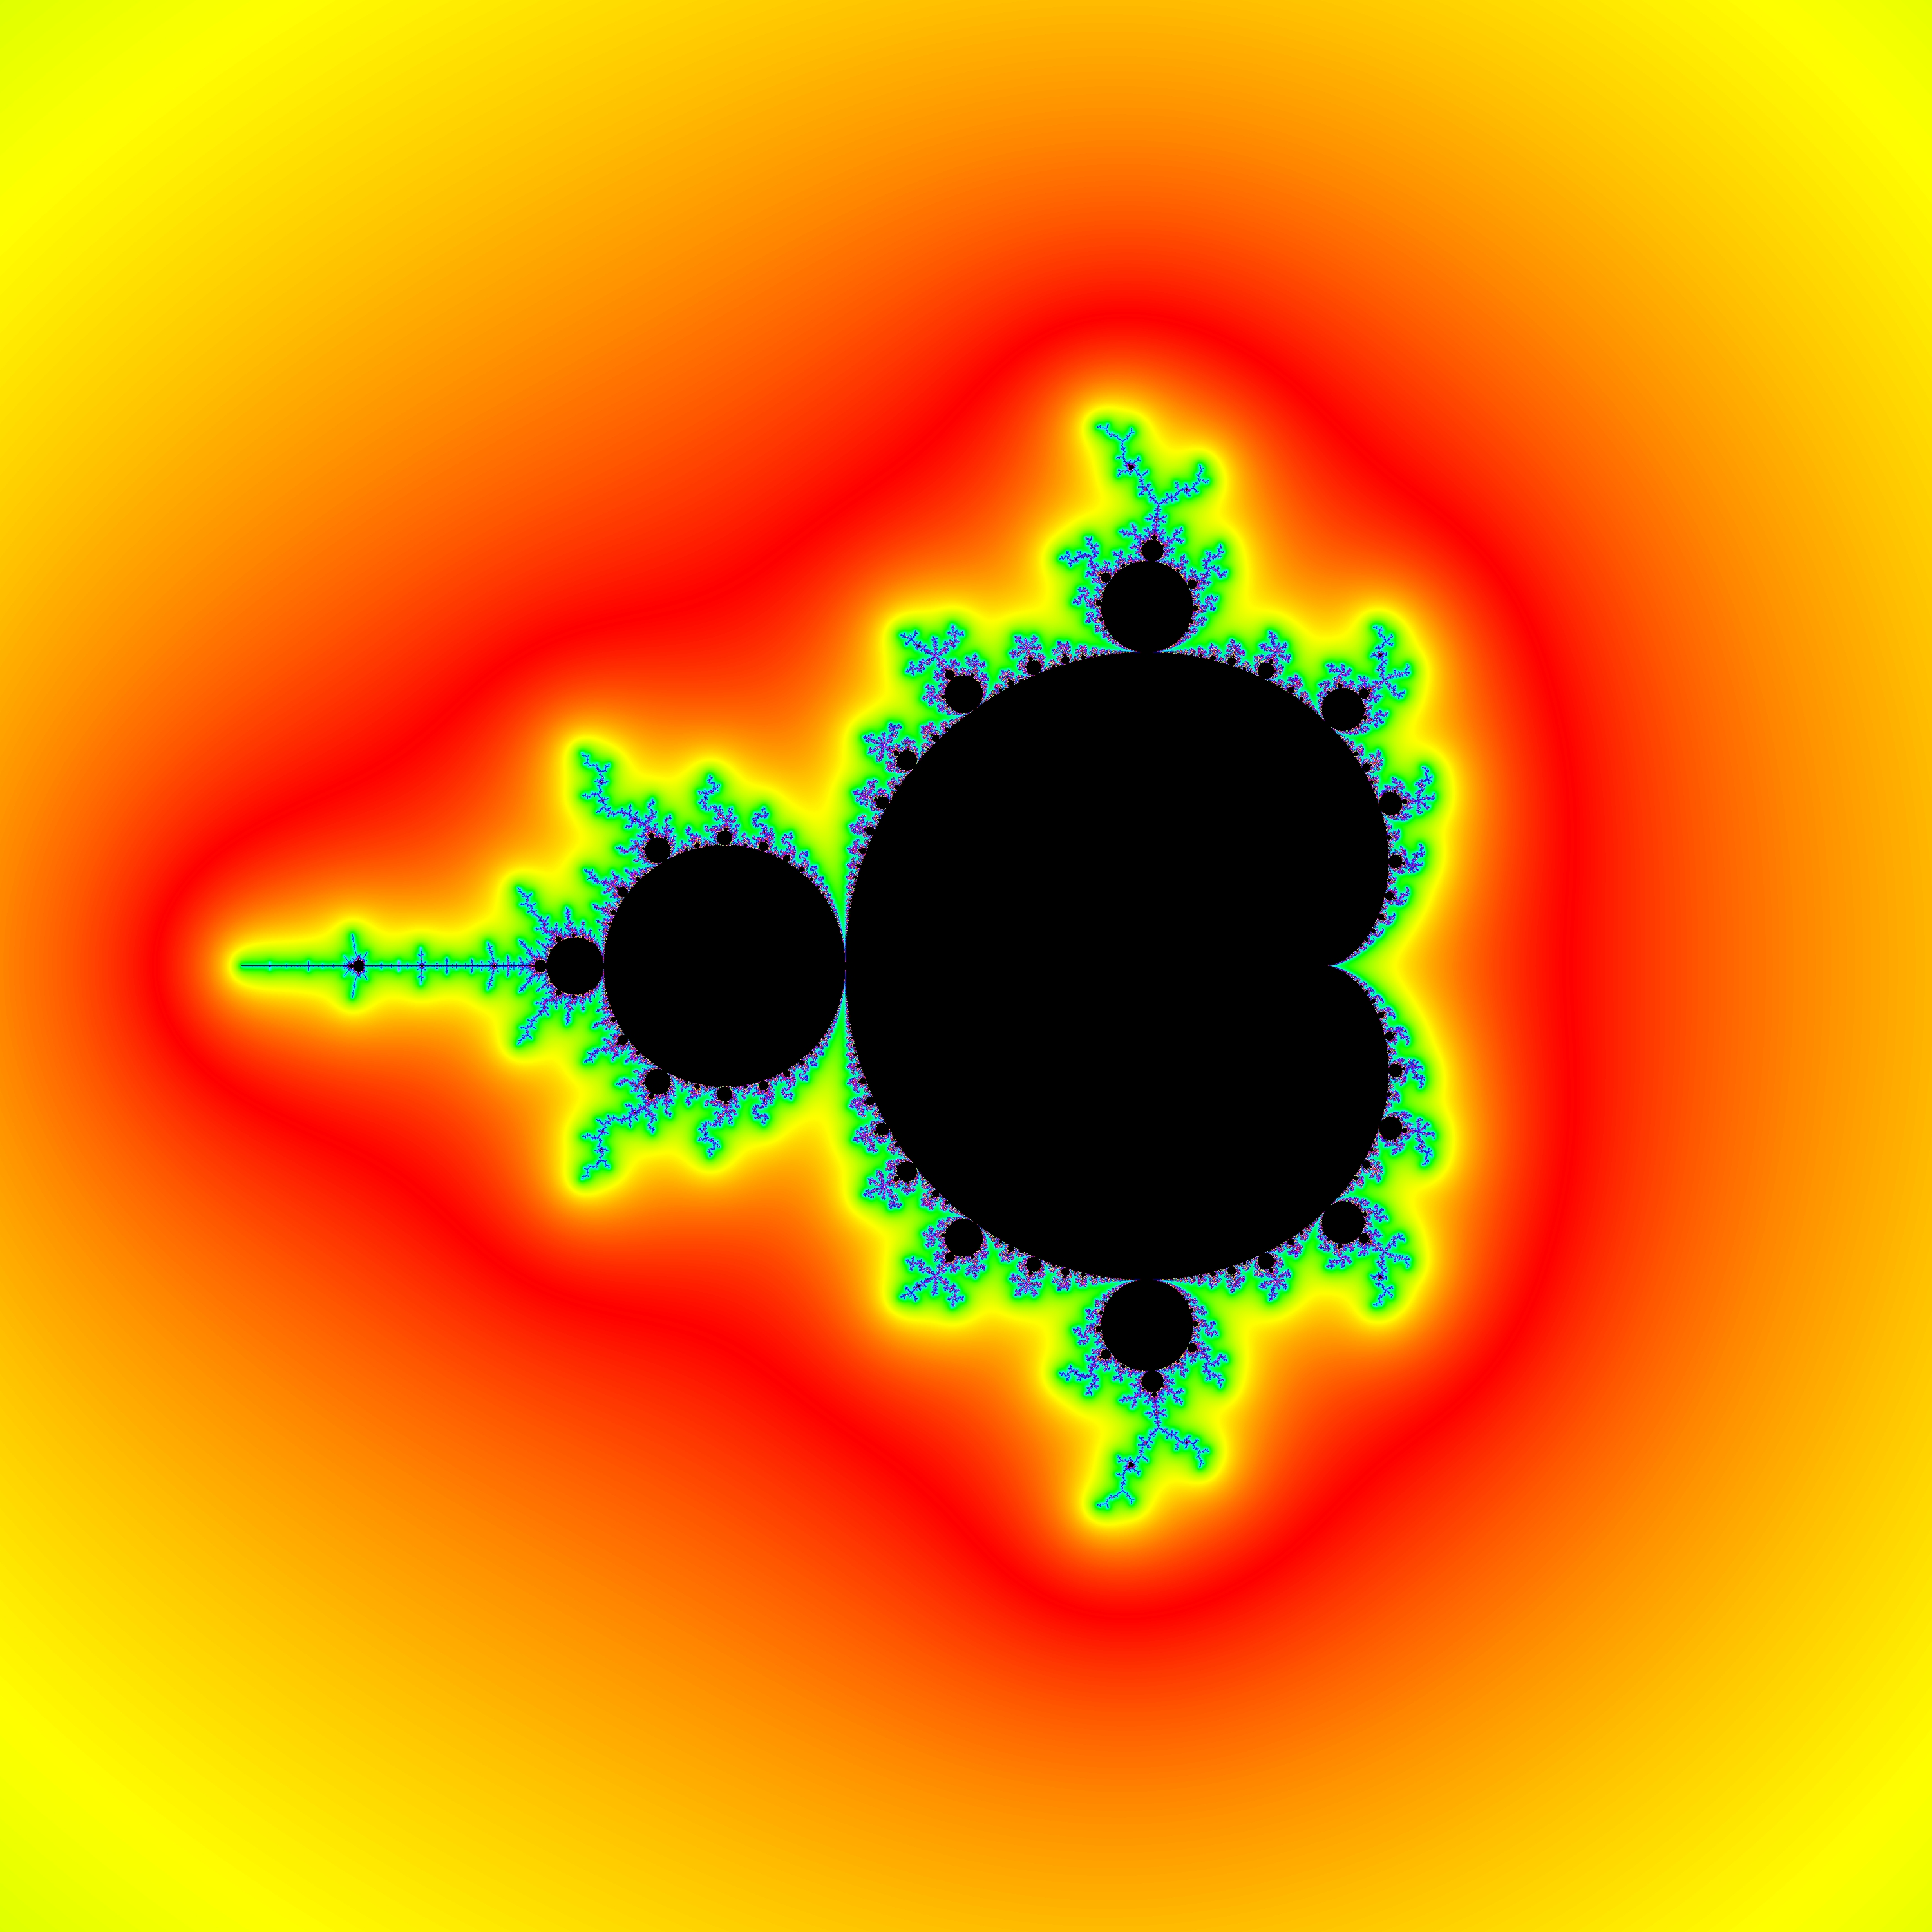
\includegraphics[width=\textwidth]{graphics/mandelbrot.jpg}
    \caption{The Mandelbrot set \(M\). Points \(z\in M\) are colored black. Other points are colored according to their estimated distances to \(\partial M\).}
    \label{mandelbrot_picture}
\end{figure}

The mandelbrot set is a fractal, which means that by zooming into the set similar patterns appearagain and again. A video\footnote{\url{https://vimeo.com/12185093}} shows zooming into the border of \(M\) reaching a zoom factor of \(2^{760}\). The video is not art nor kitsch; it is a visualisation of \(M\) created solely out of its definition. The colors indicate how fast a point \(c\notin M\) diverges from zero. (The music is not generated from the definition of \(M\).)

According to a 1991 publication\footnote{\url{https://arxiv.org/abs/math/9201282}} by M. Shishikura, the Hausdorff dimension of the border of \(M\) is two. The precise definition of Hausdorff dimension is complicated, but it can be understood heuristically.

When measuring the volume of a set in \(\RR^3\), we cover the set with small balls and add their volumes together. The smaller balls we use, the more precise estimate of the volume we get. A reasonable three-dimensional object has positive volume. On the other hand, its border which is a two-dimensional object has zero volume since the volume of a ball is proportional to the cube of its radius \(r\) but the number of needed balls is proportional to \(r^2\). Therefore, as we use smaller and smaller balls the estimate of the volume goes to zero.

However, we can measure the area of the border by artificially changing the formula for calculating the volume of a ball from being proportional to \(r^3\) to being proportional to \(r^2\). If we want to calculate the length of a one-dimensional object, change it to being proportional to \(r\). If you use too low \(x\) in \(r^x\), you get \(\infty\). Each set has its own correct \(x\), the Hausdorff dimension of the set.

Sets we study usually have \(x\in\NN\). The Hausdorff dimensions of a rock, a piece of paper and a length of wire are \(3\), \(2\) and \(1\). An esoteric set may have non-integer Hausdorff dimension. Usually the Hausdorff dimension of the border of a set \(X\) is less than the one of \(X\) by one.

\(M\) and \(\partial M\) has the same Hausdorff dimension, two. It means that \(\partial M\) must be very wrinkled. It implies that no matter how deep we zoom into \(\partial M\), we will always see complex patterns.%define \partial M
% note that wikipedia has decent articles of almost all mathematical concepts
% cardinality of C

Let me collect the sdcs. We have the countable sets \(\NN\), \(\ZZ\) and \(\QQ\) of cardinality \(\aleph_0\) and uncountable sets \(\RR\) and \(\CC\) of cardinality \(2^{\aleph_0}\).

\section{Rigor}

 In other words: do we embrace the Axiom of Choice or not? It seems obvious, but well-ordering seems ridiculous. Furthermore, AxC implies bizarre things like Banach-Tarski paradox.

The point of math: if we define precise axioms and prove theorems from those axioms carefully, then we know that every time we have a situation in which those axioms hold, then also the theorems hold. For example, a bent sheet of metal satisfies the definition of a 2-dimensional Riemannian manifold, so we know that it's curvature at any point can be characterized with two real numbers, and that curvature satisfies the Bianchi identities.

groups. examples: Z, R, SO(3) and its simply connectedness (dirac's belt), SU(2) (maybe), linear algebra

do parallel lines continue to be parallel? parallel axiom. manifolds. results: curvature tensor, bianchi identities.

\section{Some axiomatizations}


Can we comb a hairy ball? No, there will be at least one cowlick-if the surface of the ball is two-dimensional, \(S^2\). Clearly we can comb \(S^1\). We can also imagine spheres of higher dimensionality. Which spheres we can comb, and which we can't? We need math. More precisely, we need topology and algebra.

Is SO(3) simply connected? Parametrize a tau-rotation with a belt. You'll notice that you can't deform this parameterization (path) into the identity: SO(3) is not simply connected. Dirac's belt trick: the belt encodes information of how the buckle has been rotated into it's position. Electrons remember this??

%\section{Mechanics}

%\chapter{Our space and time}

%\chapter{To deduce and compute}

%\chapter{Linear algebra}




\end{document}
